\documentclass[a4paper,12pt]{article}

\usepackage[spanish,mexico]{babel}
\usepackage[T1]{fontenc}
\usepackage[top=2.5cm,bottom=2.5cm,left=3.25cm,right=3.25cm]{geometry}
\usepackage{hyperref}
\title{Planificación en STRIPS/PDDL}
\makeatletter
\let\newtitle\@title
\makeatother
\usepackage[round]{natbib}
\usepackage{multirow}
\usepackage[table]{xcolor}
\definecolor{UnirLight}{HTML}{E6F4F9}
\definecolor{UnirDark}{HTML}{0098CD}
\arrayrulecolor{UnirDark}
\usepackage{caption}
\usepackage{subcaption}
\usepackage{titlesec}
\usepackage{fancyhdr}
\pagestyle{fancy}
\renewcommand{\headrulewidth}{0pt}
\headheight=45pt
\setlength{\footskip}{64pt}
\linespread{1.3}
\usepackage[sfdefault,lf]{carlito}
\lhead{}
\chead{
  \begin{tabular}{|c|l|c|}
    \hline
    \rowcolor{UnirLight}
    \textcolor{UnirDark}{Asignatura} & \textcolor{UnirDark}{Datos del alumno} & \textcolor{UnirDark}{Fecha} \\
    \hline
    \multirow{2}{12em}{\textbf{Razonamiento y planificación automática}} & Apellidos: Domínguez Espinoza & \multirow{2}{5em}{\today} \\
    & Nombre: Edgar Uriel & \\
    \hline
    \end{tabular}}
\rhead{}
\lfoot{}
\cfoot{}
\rfoot{\makebox(70,56)[t]{\textcolor{UnirDark}{Actividades}}
  \colorbox{UnirDark}{
    \makebox(10,56)[t]{
      \textcolor{white}{\thepage}}}}
\usepackage[color={[gray]{0.5}}, angle=90,fontsize=9pt,anchor=lb,pos={0.03\paperwidth,0.95\paperheight}]{draftwatermark}
\SetWatermarkText{{\copyright} Universidad Internacional de La Rioja (UNIR)}
\titleformat*{\section}{\color{UnirDark}\normalsize\bfseries}
\titleformat*{\subsection}{\color{UnirDark}\normalsize\bfseries}
\usepackage{listings}
\definecolor{gray97}{gray}{.97}
\definecolor{gray75}{gray}{.75}
\definecolor{gray45}{gray}{.45}
\lstset{ frame=Ltb,
  framerule=0pt,
  aboveskip=0.5cm,
  framextopmargin=3pt,
  framexbottommargin=3pt,
  framexleftmargin=0.4cm,
  xleftmargin=6mm,
  framesep=0pt,
  rulesep=.4pt,
  columns=fixed,
  backgroundcolor=\color{gray97},
  rulesepcolor=\color{black},
  stringstyle=\ttfamily,
  showstringspaces = false,
  basicstyle=\small\ttfamily,
  commentstyle=\color{gray45},
  keywordstyle=\bfseries,
  numbers=left,
  numbersep=15pt,
  numberstyle=\tiny,
  numberfirstline = false,
  breaklines=true,}
\lstnewenvironment{listing}[1][]
{\lstset{#1}\pagebreak[0]}{\pagebreak[0]}
\lstdefinestyle{consola}
{basicstyle=\scriptsize\bf\ttfamily,
  backgroundcolor=\color{gray75},}
\lstdefinestyle{Lisp}
{language=Lisp}
\hypersetup{
  pdfauthor={Edgar Uriel Domínguez Espinoza},
  pdftitle={Planificación en STRIPS/PDDL},
  pdfkeywords={strips, pddl, planificación, ff, downward, lpg-td},
  pdfsubject={Razonamiento y planificación automática},
  pdfcreator={GNU Emacs 27.2},
  pdflang={"Spanish"}}

\begin{document}

\textcolor{UnirDark}{\LARGE\bfseries\newtitle}

\section{Introducción}

En trabajos anteriores se ha explorado el estado del arte en el área de planificadores automáticos para la Inteligencia Articial (IA). En el presente texto se retoma el uso de los planificadores para resolver problemas expresados en STRIPS/PDDL.

\section{Marco referencial}

\section{Dominio y problemas}

\begin{figure}
     \centering
     \begin{subfigure}[b]{0.45\textwidth}
         \centering
         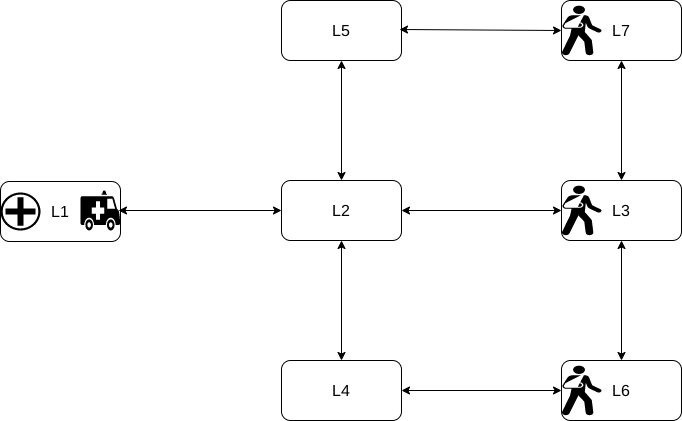
\includegraphics[width=\textwidth]{im/variante01}
         \caption{Variante 1}
         \label{fig:original}
     \end{subfigure}
     \hfill
     \begin{subfigure}[b]{0.45\textwidth}
         \centering
         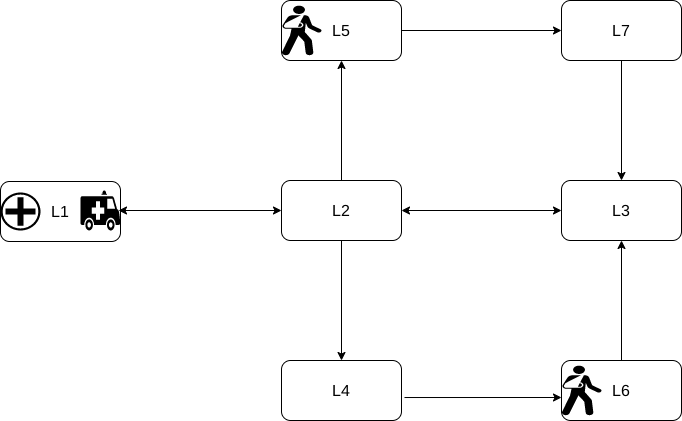
\includegraphics[width=\textwidth]{im/variante02}
         \caption{Variante 2}
         \label{fig:var1}
     \end{subfigure}
     \hfill
     \begin{subfigure}[b]{0.45\textwidth}
         \centering
         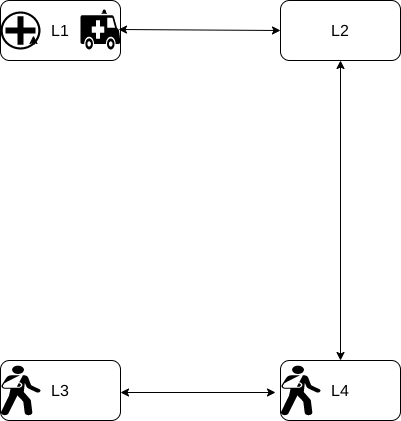
\includegraphics[width=\textwidth]{im/original}
         \caption{Problema original}
         \label{fig:var2}
     \end{subfigure}
        \caption{Problemas resueltos}
        \label{fig:problemas}
\end{figure}

\lstinputlisting[language=Lisp, numbers=left]{domain.pddl}
\lstinputlisting[language=Lisp, numbers=left]{problem01.pddl}
%% \lstinputlisting[language=Lisp, numbers=left]{problem02.pddl}
%% \lstinputlisting[language=Lisp, numbers=left]{problem03.pddl}

\section{Resultados y comparación}

\lstinputlisting[style=consola, numbers=left]{out/p1-ff}
\lstinputlisting[style=consola, numbers=left]{out/p1-lpg-td_1.SOL}
\lstinputlisting[style=consola, numbers=left]{out/p1-solver.planning.domains}
\lstinputlisting[style=consola, numbers=left]{out/p1-solver.planning.domains-time}
\begin{lstlisting}[style=consola, numbers=left]
  Solution found!
  Actual search time: 0s [t=0.00119607s]
  move hospital l2 (1)
  move l2 l4 (1)
  move l4 l3 (1)
  getinto patient1 l3 ambulance (1)
  move l3 l4 (1)
  move l4 l2 (1)
  move l2 hospital (1)
  getout patient1 hospital ambulance (1)
  move hospital l2 (1)
  move l2 l4 (1)
  getinto patient2 l4 ambulance (1)
  move l4 l2 (1)
  move l2 hospital (1)
  getout patient2 hospital ambulance (1)
  Plan length: 14 step(s).
  Plan cost: 14
  Expanded 30 state(s).
  Reopened 0 state(s).
  Evaluated 40 state(s).
  Evaluations: 80
  Generated 69 state(s).
  Dead ends: 0 state(s).
  Expanded until last jump: 25 state(s).
  Reopened until last jump: 0 state(s).
  Evaluated until last jump: 33 state(s).
  Generated until last jump: 58 state(s).
  Number of registered states: 40
  total successors before partial-order reduction: 69
  total successors after partial-order reduction: 69
  Search time: 0s
  Total time: 0.00119607s
  Solution found.
  Peak memory: 4960 KB
\end{lstlisting}

\section{Conclusión}

\bibliographystyle{apalike}
\bibliography{mexmiart04t9lab}
\end{document}
